\section{遺伝的アルゴリズム}
遺伝的アルゴリズム(GA)とは,適用範囲の非常に広い,生物の進化を模倣した学習的アルゴリズムである\cite{遺伝的アルゴリズム}.すなわち何万年,何億年もかけて生物の特徴が進化してきたような遺伝的法則を工学的な手法にモデル化し,また参考にしてタスクを解くものである.自然界における生物の進化過程においては,ある世代を形成している個体の集合,すなわち個体群の中で環境に適している個体が高い確率で生き残り,生き残った個体は交叉や突然変異によって次の世代の個体群が形成される.

\subsection{本論文における基本的動作}
本論文において,新しく個体を形成する際に交叉は使用しない.以降本論文で用いる遺伝的アルゴリズム変則GAと呼ぶ.図は変則GAの動作を流れを表している.

\begin{figure}[h]
    \begin{center}
        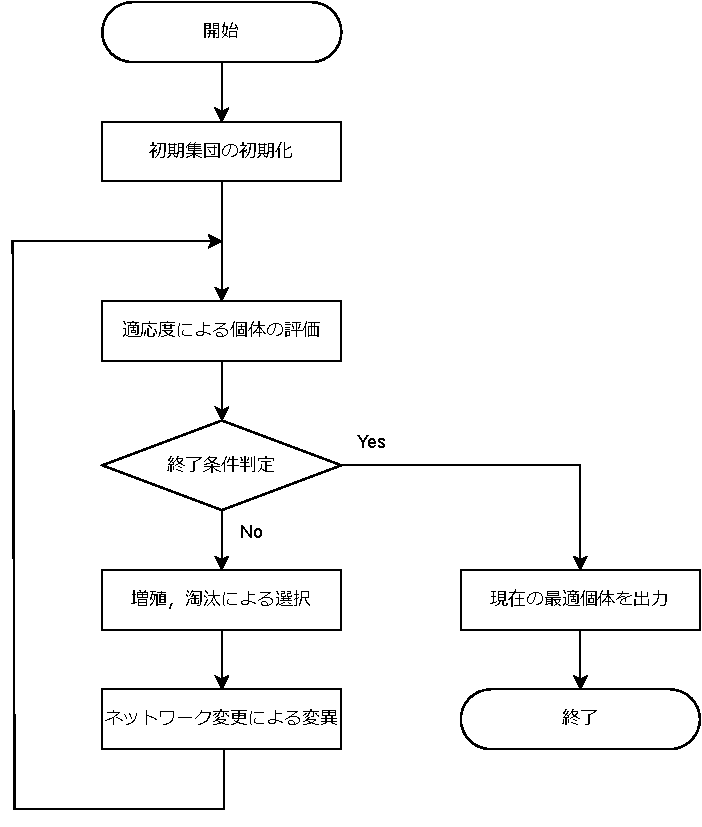
\includegraphics[scale=0.8]{img/expga.pdf}
        \caption{変則GAの概要}
    \end{center}
\end{figure}


\begin{enumerate}
    \item 初期化 \\
    ランダムな性質を持つ個体を $ N $ 個生成し,初期世代の個体群を設定する.

    \item 評価 \\
    各個体についてタスクを解かせ,その進捗により適応度を測定する.

    \item 終了判定 \\
    終了条件を満たしていれば,その時に得られる最適個体を問題の準最適解として出力する.

    \item 選択 \\
    各個体に対応する適応度により並べ替え,適応度の低い個体は淘汰され,適応度の高い個体は増殖する.

    \item 変異 \\
    設定された突然変異の設定により変異を行い,新しい個体群を生成する.変異を行った後の個体群は次世代の個体群として再度評価される.
\end{enumerate}

終了判定には最良個体の適応度や個体群の平均の適応度を参照する場合が多いが,本論文ではあらかじめ設定した世代数を超えたときにのみ終了判定が真になり,プログラムは終了する.また,変異をする過程でエリート保存選択を実行する.これは非常に優れた個体は変異をする前の状態のほうが変異をした後の状態よりも優れている見込みが大きいことから,個体に対して変異を行わず,全く同じ状態の個体を次世代に残す手法である.エリート保存選択は,むやみに変異をして優良個体の遺伝子を破壊しないことにつながる.

\subsection{ルーレット選択}
ルーレット選択は,個体群の中の各個体の適応度とその総計を求めて,適応度の総計に対する各個体の割合を選択確率として個体を選択するという基本的な考えに基づいている\cite{遺伝的アルゴリズム}.すなわち,ルーレット選択では,個体 $ s_i $ の適応度 $ f{s_i} $ と個体群の総計を求め,個体 $ s_i $ が選択される確率を

\begin{equation}
    P_i = \frac{f(s_i)}{\sum^N_{j=1} f(s_j)}
\end{equation}

として個体の確率的に選択する.このようなルーレット選択のアルゴリズムは,次のように要約される.

\begin{enumerate}
    \item 世代 $ t $ の個体群 $ X(t) $ の中の $ N $ 個の個体の適応度 $ f_i $ とその総計 $ f_{sum} = \sum^N_{i=1} f_i $ を求める.

    \item 区間[0, 1]の乱数 $ rand $ を発生させ, $ s = rand \times f_{sum} $ とする.

    \item $ \sum^k_{i=1} f_i \geq s $ となるような最小の $ k $ を求めて, $ k $ 番目の個体を世代 $ t+1 $ に生き残る個体の候補とする.

    \item 候補となる個体数が $ N $ になるまで2, 3を繰り返す.
\end{enumerate}

本論文ではルーレット選択を個体の変異先を選択する際に用いる.同じ構造を持つネットワークの,ひとつのノードの活性化関数のみを変更し,この出力が小さいほど $ f_i $ が大きいことになる.
